\chapter{Residual Noise Analysis and Discussion}

\section{Motivation}

The main quantitative results show that CTRestormer 21500 achieves strong PSNR, SSIM, and RMSE. However, medical image denoising should not be judged only by aggregate image quality metrics. A denoised image can look cleaner because noise has been removed, but it can also look cleaner because the model has suppressed subtle anatomical texture. For this reason, this thesis studies residual maps.

The residual analysis asks a direct question: what did the model remove from the low-dose input? The estimated true residual is \(x-y\), where \(x\) is the LDCT input and \(y\) is the NDCT target. The removed residual is \(x-\hat{y}\), where \(\hat{y}\) is the model prediction. If the removed residual resembles the estimated true residual and contains limited edge-like anatomical structure, the model is more likely to be removing noise rather than simply smoothing the image.

\section{Residual Map Results}

Figure \ref{fig:pred_standard} presents the standardized prediction comparison for L506\_88. The CTformer prediction in this residual study uses the updated 100000-iteration checkpoint. The figure separates the visual comparison from the residual analysis so that the reader can first inspect image-level restoration quality. Figure \ref{fig:removed_residuals} then focuses only on the residual removed by each model. This separation is important because a denoised image may look acceptable even when the removed residual contains structure-related signal.

\begin{figure}[!htbp]
    \centering
    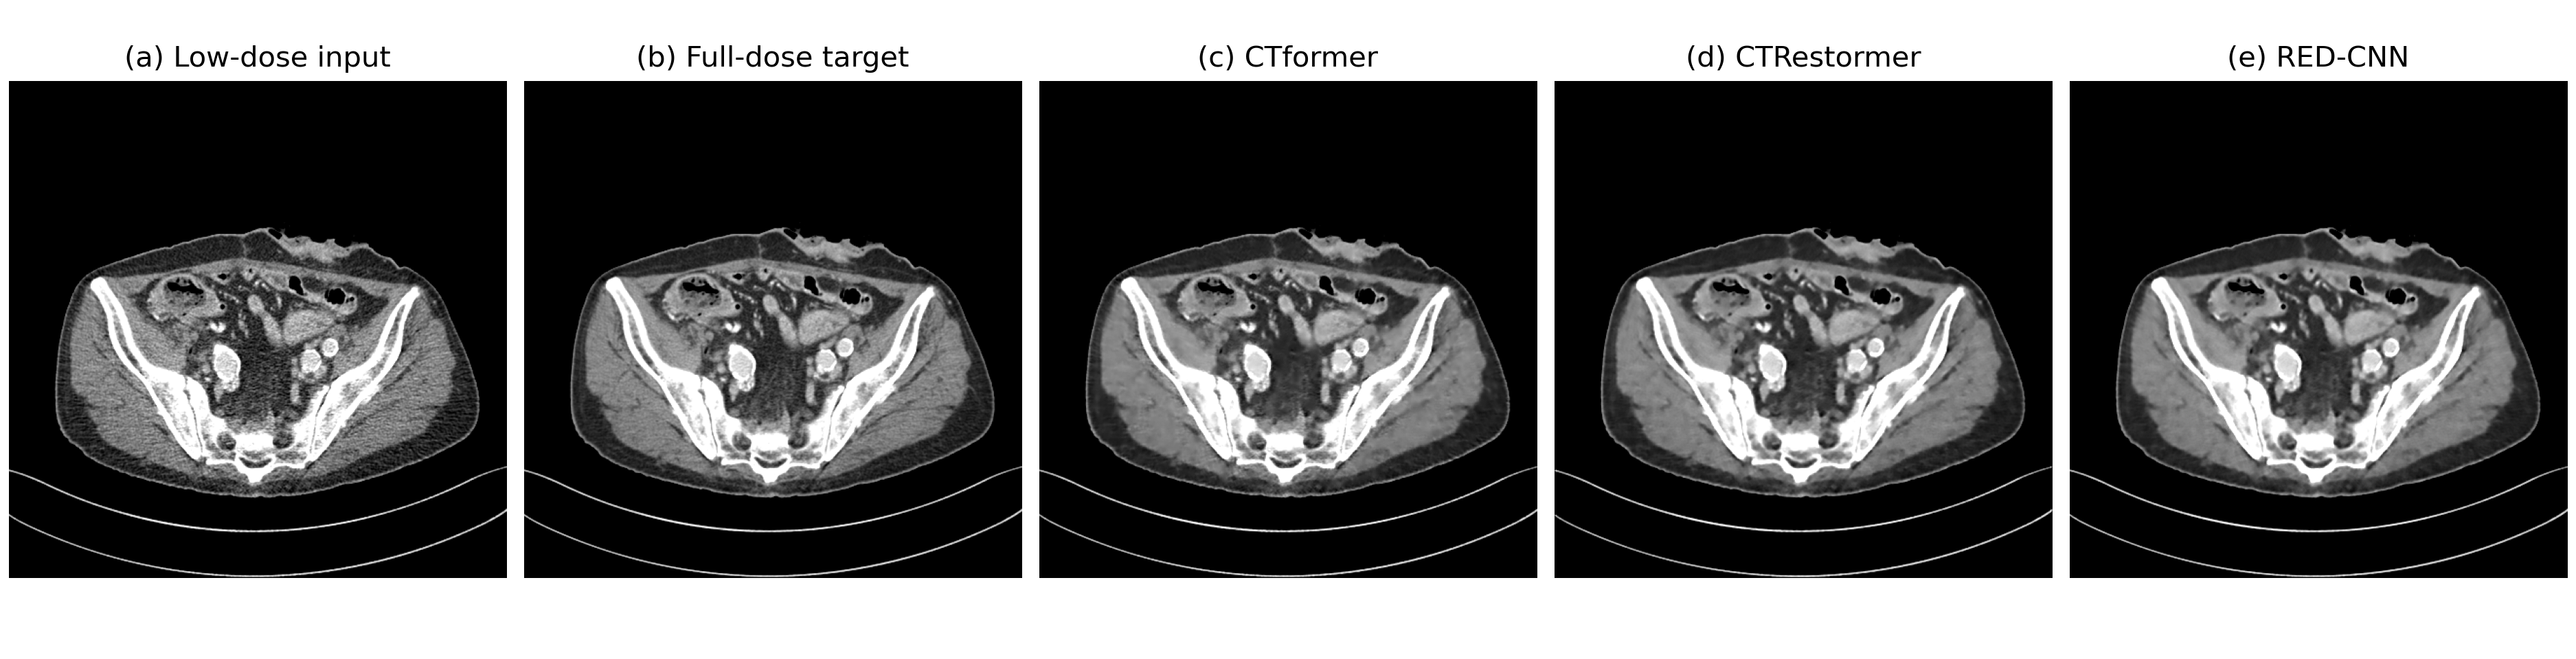
\includegraphics[width=0.95\textwidth]{images/L506_88_prediction_comparison_standard.png}
    \caption{Standardized prediction comparison for L506\_88 using a shared CT display window. CTformer uses the updated 100000-iteration checkpoint.}
    \label{fig:pred_standard}
\end{figure}

\begin{figure}[!htbp]
    \centering
    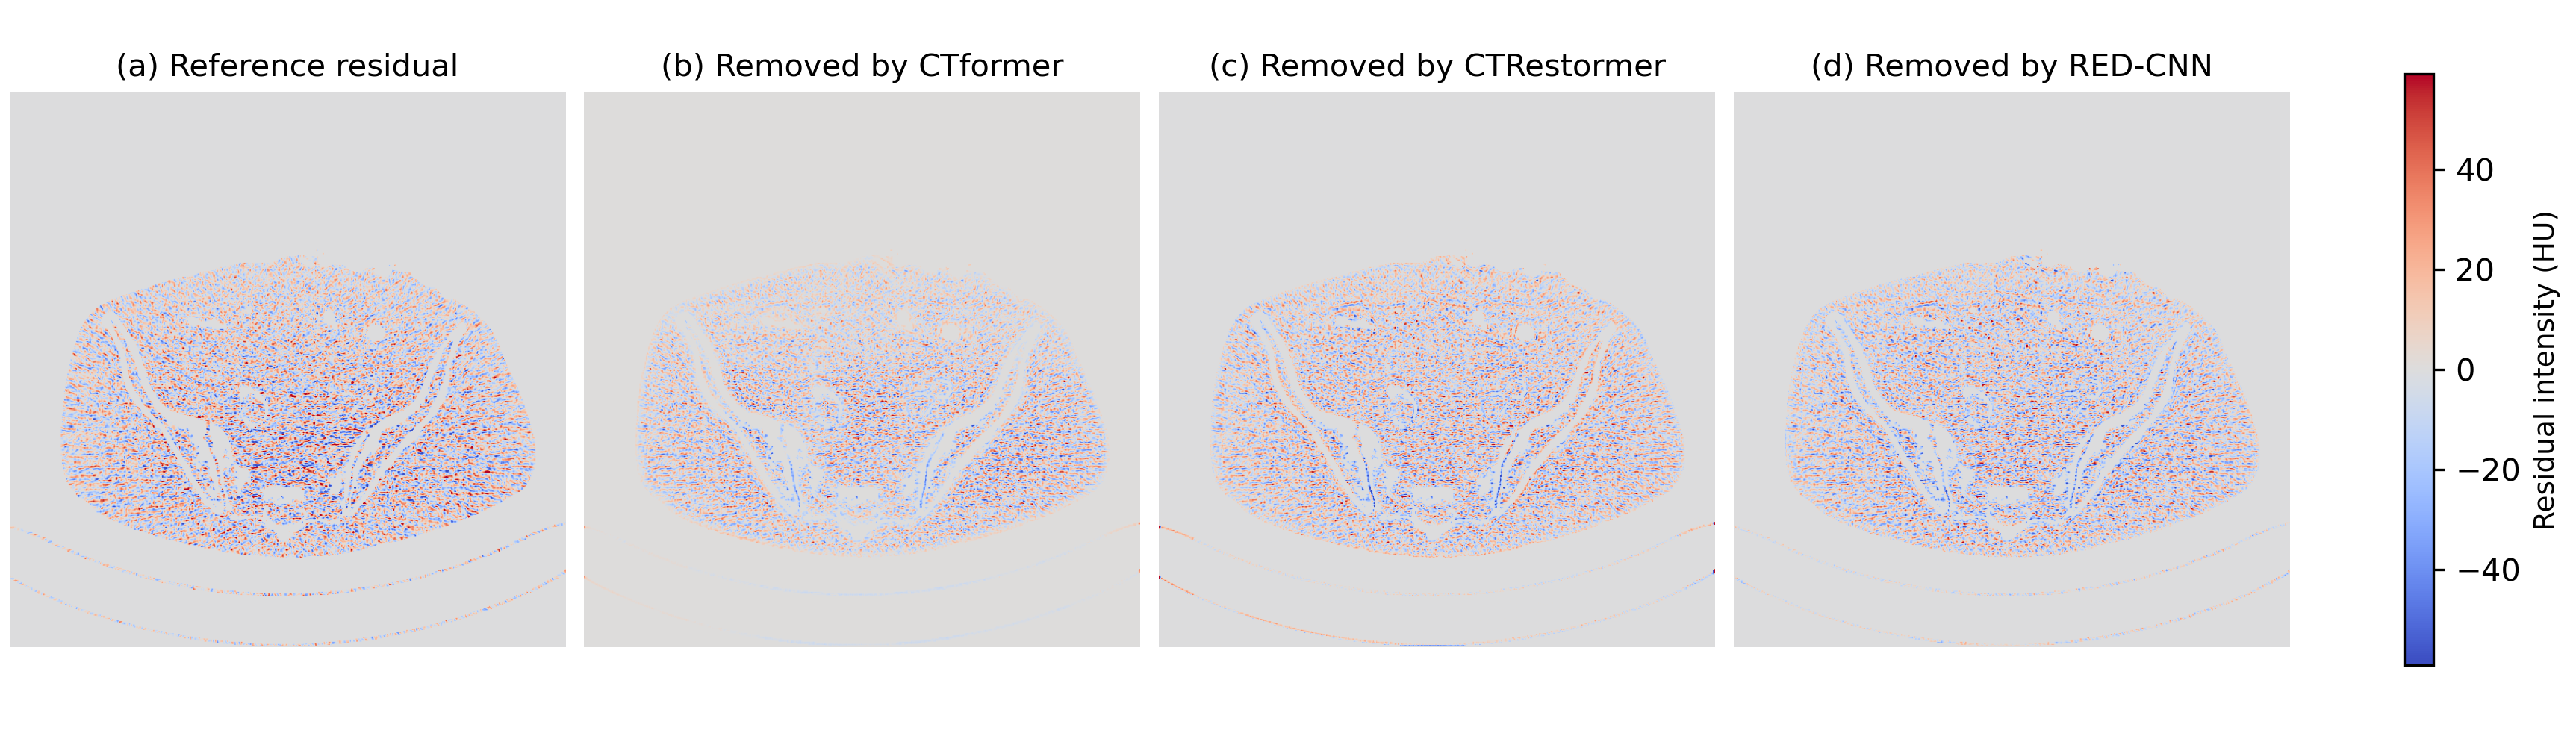
\includegraphics[width=0.95\textwidth]{images/L506_88_removed_residuals_standard.png}
    \caption{Removed residual maps computed as input minus prediction. The panels use a shared diverging residual scale to compare removal strength.}
    \label{fig:removed_residuals}
\end{figure}

The residual maps show different denoising behaviors. CTformer removes a more conservative residual, while CTRestormer and RED-CNN remove stronger residual patterns. Stronger removal is not automatically better; it must be interpreted together with prediction error and edge leakage. If the removed residual contains obvious anatomical edges, the denoising model may be suppressing structure. If the removed residual is mainly noise-like texture, the behavior is more desirable.

\section{Prediction Error and Residual Statistics}

Figure \ref{fig:prediction_error} shows the prediction error maps for L506\_88. These maps represent \(\hat{y}-y\), so they show what remains different from the NDCT target after denoising. Figure \ref{fig:residual_bars} summarizes residual correlation and edge leakage. Table \ref{tab:residual_stats} reports the residual statistics.

\begin{figure}[!htbp]
    \centering
    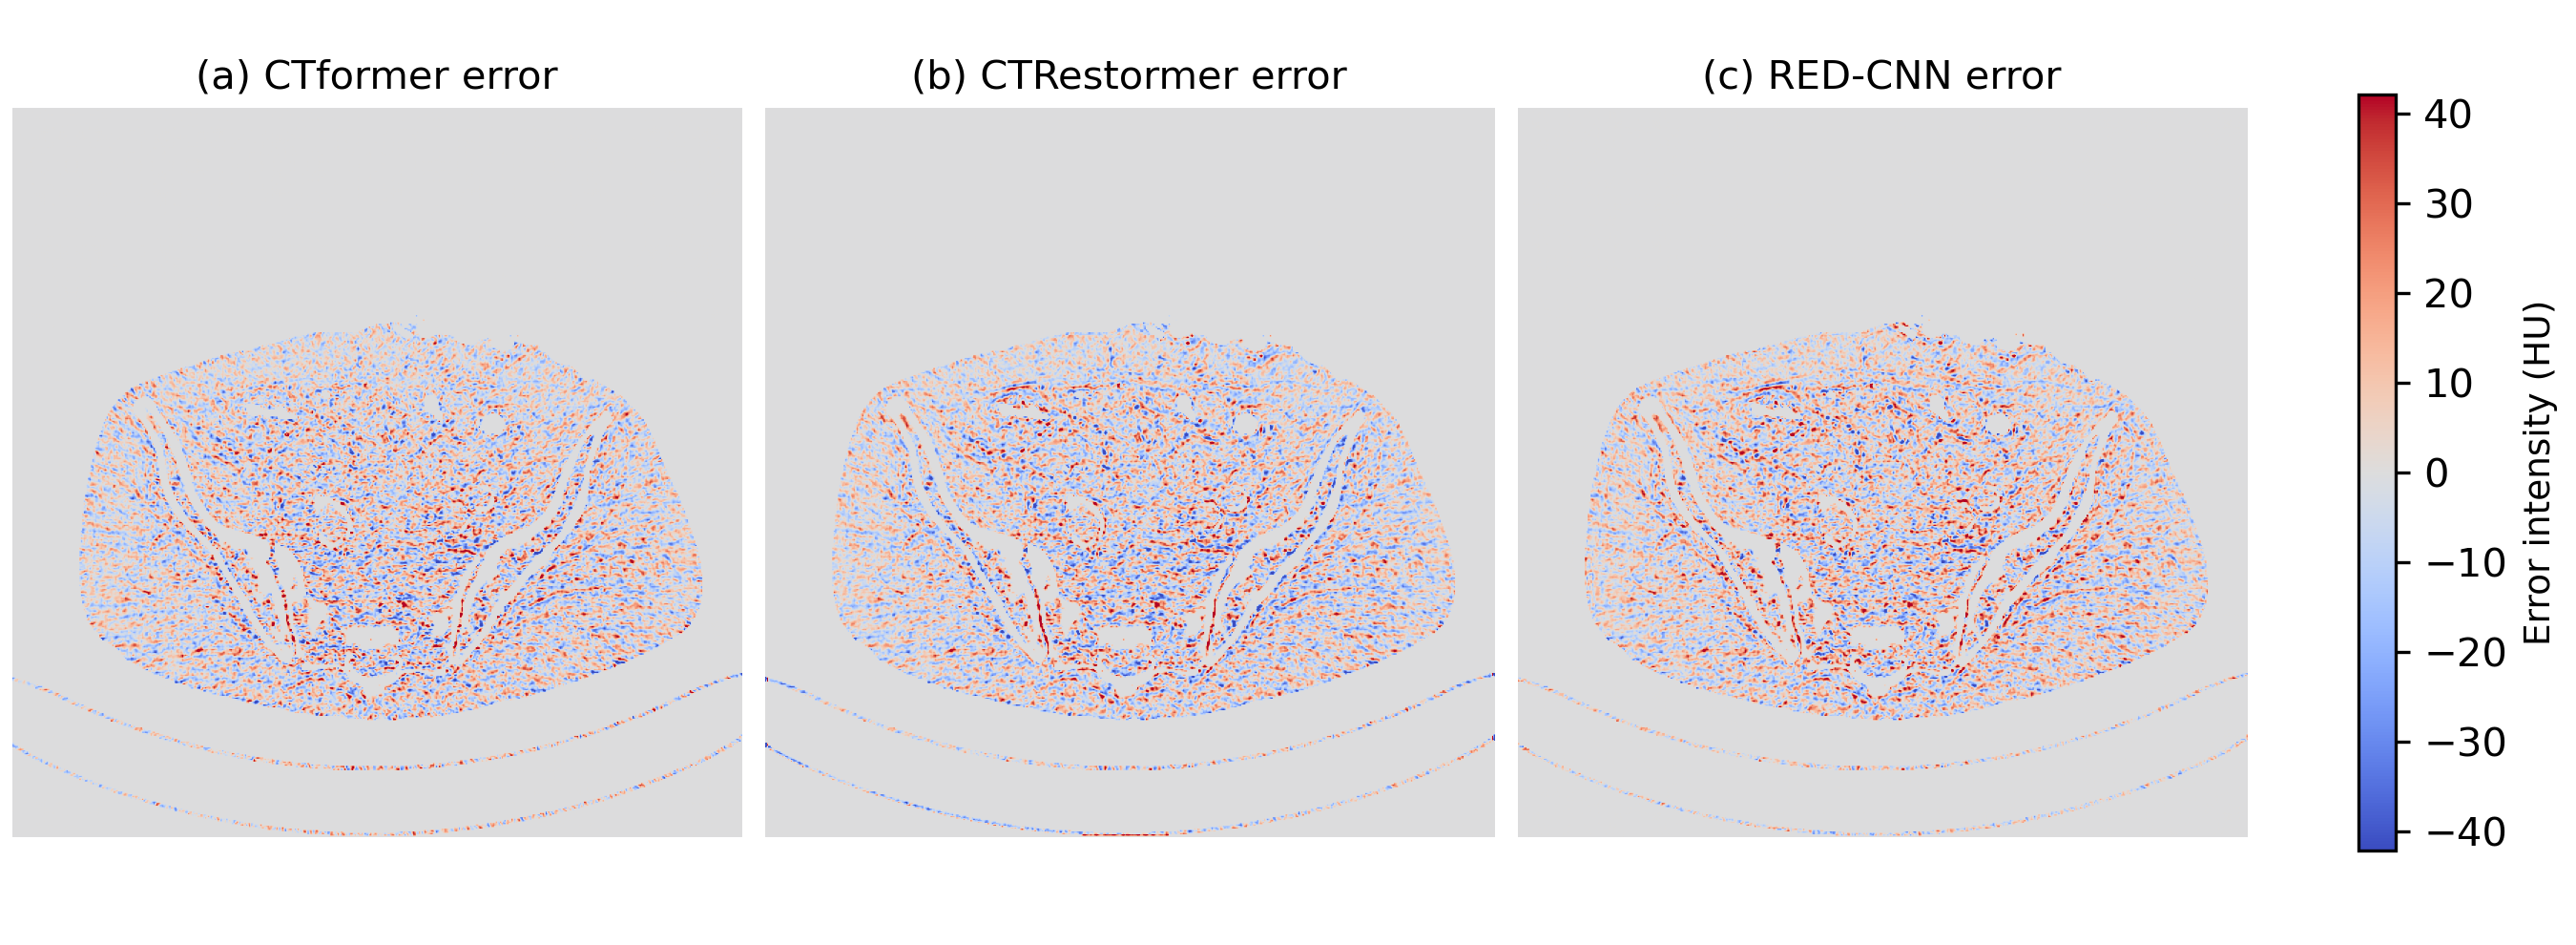
\includegraphics[width=0.95\textwidth]{images/L506_88_prediction_errors_standard.png}
    \caption{Prediction error maps computed as prediction minus target for L506\_88.}
    \label{fig:prediction_error}
\end{figure}

\begin{figure}[!htbp]
    \centering
    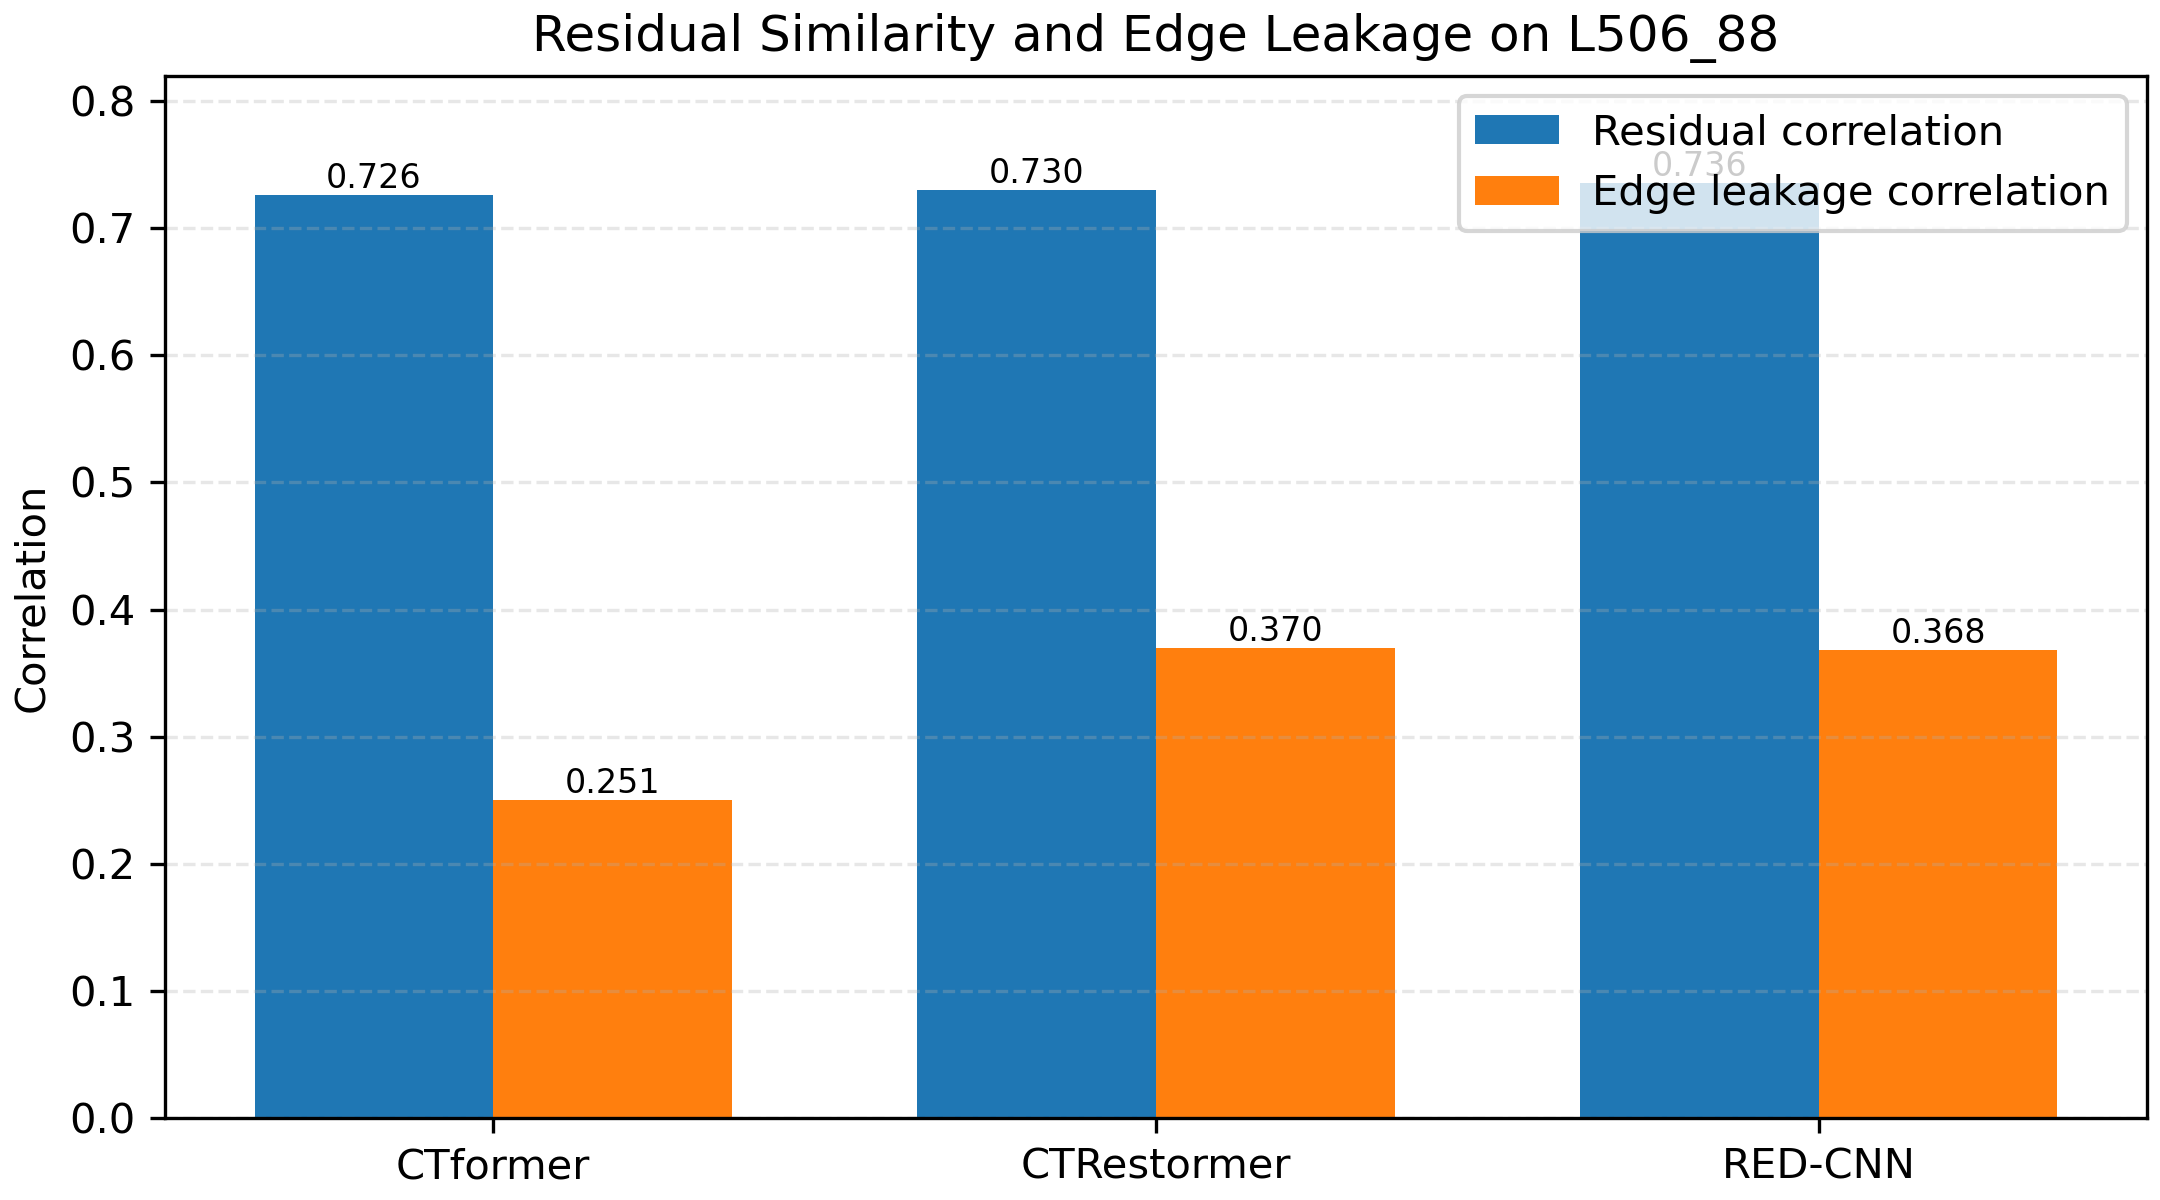
\includegraphics[width=0.75\textwidth]{images/L506_88_residual_metrics_bar_standard.png}
    \caption{Residual correlation and edge leakage comparison for the representative L506\_88 slice.}
    \label{fig:residual_bars}
\end{figure}

\begin{table}[!htbp]
    \centering
    \caption{Residual noise statistics for representative slice L506\_88.}
    \renewcommand{\arraystretch}{1.25}
    \small
    \begin{tabular}{lccccc}
        \hline
        Model & Corr. & Edge & Std & Removed MAE & Error MAE \\
        \hline
        CTformer 100000 & 0.7259 & 0.2506 & 9.8406 & 4.3490 & 4.1493 \\
        \hline
        CTRestormer & 0.7300 & 0.3699 & 11.3863 & 5.2081 & 4.1636 \\
        \hline
        RED-CNN & 0.7358 & 0.3683 & 11.7800 & 5.3967 & 4.1823 \\
        \hline
    \end{tabular}
    \label{tab:residual_stats}
\end{table}

The three models have residual correlations around 0.72 to 0.74, suggesting that their removed residuals are substantially related to the estimated LDCT residual. CTformer has the lowest edge leakage, which suggests more conservative residual removal. CTRestormer and RED-CNN remove stronger residuals and have similar edge leakage values. This supports a balanced interpretation: CTRestormer achieves strong image quality metrics, but its residual behavior should still be inspected for possible structure suppression.

\section{Histogram and Frequency Analysis}

Residual histograms and power spectra provide complementary information. The histogram shows the distribution of removed residual values, while the power spectrum shows how residual energy is distributed across spatial frequencies. Figures \ref{fig:histogram} and \ref{fig:spectrum} summarize these two views for L506\_88.

\begin{figure}[!htbp]
    \centering
    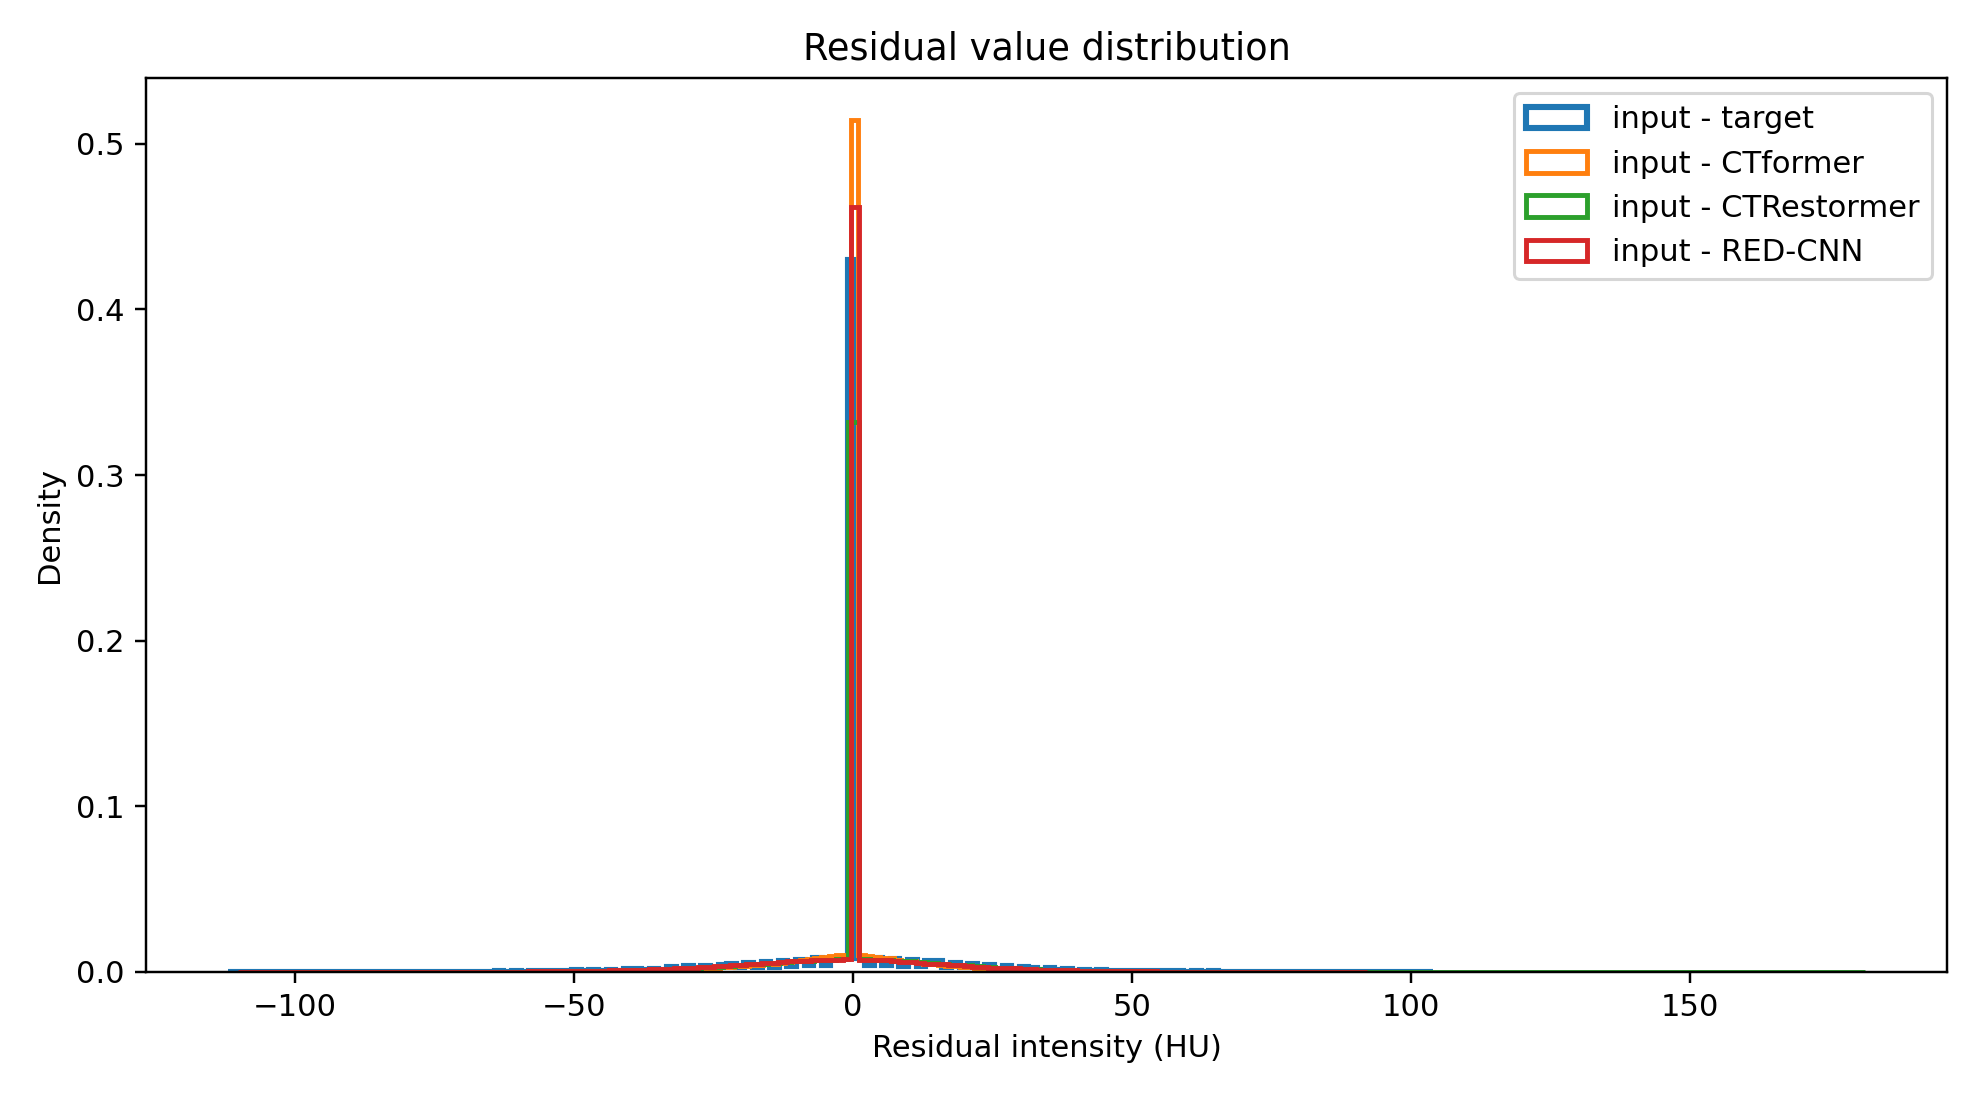
\includegraphics[width=0.78\textwidth]{images/L506_88_residual_histogram.png}
    \caption{Histogram of removed residual values for L506\_88.}
    \label{fig:histogram}
\end{figure}

\begin{figure}[!htbp]
    \centering
    
\includegraphics[width=0.78\textwidth]{images/L506_88_residual_power_spectrum.png}
    \caption{Radially averaged residual power spectrum for L506\_88.}
    \label{fig:spectrum}
\end{figure}

These plots help distinguish denoising strength from denoising quality. A method that removes more residual energy may produce a smoother output, but whether the removed energy is desirable depends on its spatial and structural characteristics. Frequency analysis is therefore useful when comparing conservative and aggressive denoising behavior.

\section{Limitations of the Residual Study}

The current residual analysis is a representative case study on slice L506\_88. It provides useful evidence, but it should not be overstated as proof over the entire dataset. A stronger final study should compute residual correlation, removed residual standard deviation, and edge leakage for all slices in the held-out L506 patient and report mean and standard deviation.

Another limitation is that \(x-y\) is only an approximation of true LDCT noise. The NDCT target is used as a reference, but it is not a perfect noise-free image. In addition, residual maps do not directly measure clinical diagnostic accuracy. A future clinical-quality study would require region-of-interest measurements, reader studies, or task-based evaluation. Therefore, this thesis uses residual analysis as model-behavior evidence, not as a direct clinical safety claim.
